

\tikzset{every picture/.style={line width=0.75pt}} %set default line width to 0.75pt        

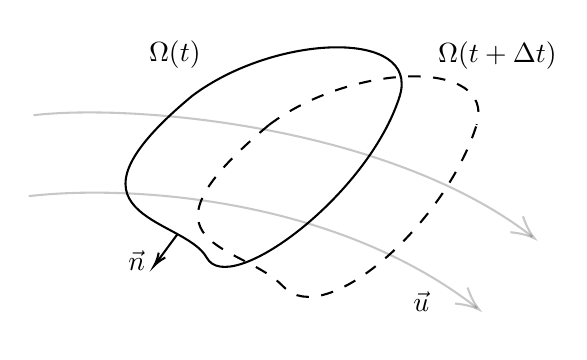
\begin{tikzpicture}[x=0.75pt,y=0.75pt,yscale=-1,xscale=1]
%uncomment if require: \path (0,232); %set diagram left start at 0, and has height of 232

%Curve Lines [id:da2643481461519446] 
\draw    (99,78.67) .. controls (139,48.67) and (208.67,46.33) .. (199,78.67) ;
%Curve Lines [id:da5225130656720315] 
\draw    (99,78.67) .. controls (63.95,107.8) and (62.56,122.37) .. (71.46,132.03) .. controls (80.58,141.94) and (100.5,146.69) .. (106,156.67) .. controls (116.86,176.38) and (184,126.67) .. (199,78.67) ;
%Curve Lines [id:da8911563864595592] 
\draw  [dash pattern={on 4.5pt off 4.5pt}]  (136,92.67) .. controls (176,62.67) and (245.67,60.33) .. (236,92.67) ;
%Curve Lines [id:da8664156559841841] 
\draw  [dash pattern={on 4.5pt off 4.5pt}]  (136,92.67) .. controls (65,151.67) and (123.21,149.67) .. (143,170.67) .. controls (162.79,191.67) and (221,140.67) .. (236,92.67) ;
%Curve Lines [id:da42970683584723535] 
\draw [color={rgb, 255:red, 0; green, 0; blue, 0 }  ,draw opacity=0.22 ][fill={rgb, 255:red, 0; green, 0; blue, 0 }  ,fill opacity=0 ]   (20.21,127) .. controls (68.63,121.36) and (167.88,127.6) .. (236.18,180.86) ;
\draw [shift={(237.21,181.67)}, rotate = 218.32] [color={rgb, 255:red, 0; green, 0; blue, 0 }  ,draw opacity=0.22 ][line width=0.75]    (10.93,-4.9) .. controls (6.95,-2.3) and (3.31,-0.67) .. (0,0) .. controls (3.31,0.67) and (6.95,2.3) .. (10.93,4.9)   ;
%Curve Lines [id:da6021980060327932] 
\draw [color={rgb, 255:red, 0; green, 0; blue, 0 }  ,draw opacity=0.22 ][fill={rgb, 255:red, 0; green, 0; blue, 0 }  ,fill opacity=0 ]   (22.54,88) .. controls (70.97,82.36) and (194.3,93.22) .. (262.85,146.53) ;
\draw [shift={(263.88,147.33)}, rotate = 218.32] [color={rgb, 255:red, 0; green, 0; blue, 0 }  ,draw opacity=0.22 ][line width=0.75]    (10.93,-4.9) .. controls (6.95,-2.3) and (3.31,-0.67) .. (0,0) .. controls (3.31,0.67) and (6.95,2.3) .. (10.93,4.9)   ;
%Straight Lines [id:da6742826970144402] 
\draw    (91.88,145.33) -- (81.73,159.06) ;
\draw [shift={(80.54,160.67)}, rotate = 306.47] [color={rgb, 255:red, 0; green, 0; blue, 0 }  ][line width=0.75]    (6.56,-1.97) .. controls (4.17,-0.84) and (1.99,-0.18) .. (0,0) .. controls (1.99,0.18) and (4.17,0.84) .. (6.56,1.97)   ;

% Text Node
\draw (76.67,50.67) node [anchor=north west][inner sep=0.75pt]   [align=left] {$\displaystyle \Omega ( t)$};
% Text Node
\draw (216,51) node [anchor=north west][inner sep=0.75pt]   [align=left] {$\displaystyle \Omega ( t+\Delta t)$};
% Text Node
\draw (204,171.33) node [anchor=north west][inner sep=0.75pt]  [color={rgb, 255:red, 0; green, 0; blue, 0 }  ,opacity=1 ] [align=left] {$\displaystyle \vec{u}$};
% Text Node
\draw (66.67,151.67) node [anchor=north west][inner sep=0.75pt]   [align=left] {$\displaystyle \vec{n}$};


\end{tikzpicture}
